\documentclass[tikz]{standalone}

%%% Packages
\usepackage{tikz}
\usetikzlibrary{arrows, positioning, shapes, snakes}


%%% Variables
\newcommand{\minwidth}{3cm}
\newcommand{\minheight}{1cm}


%%% tikzstyle
\tikzstyle{startstop} = [% start stop node
  ellipse,
  minimum width=\minwidth,
  minimum height=\minheight,
  text centered,
  draw=black,
  fill=red!20
  ]
\tikzstyle{io} = [% input output node
  trapezium,
  trapezium left angle=70,
  trapezium right angle=110,
  minimum width=\minwidth,
  minimum height=\minheight,
  text centered,
  draw=black,
  fill=blue!20
  ]
\tikzstyle{process} = [% process node
  rectangle,
  minimum width=\minwidth,
  minimum height=\minheight,
  text centered,
  draw=black,
  fill=orange!20
  ]
\tikzstyle{decision} = [% decision node
  diamond,
  minimum width=\minwidth,
  minimum height=\minheight,
  text centered,
  draw=black,
  fill=green!20
  ]
\tikzstyle{arrow} = [% arrow format
  thick,
  ->,
  >=stealth
  ]


%%%%%%%%%%%%%%%%%%%%%%%%%%%%%%%%%%%%%%%%%%%%%%%%%%%%%%%%%%%%%%%%%%%%%%%%%%%%%%%
\begin{document}

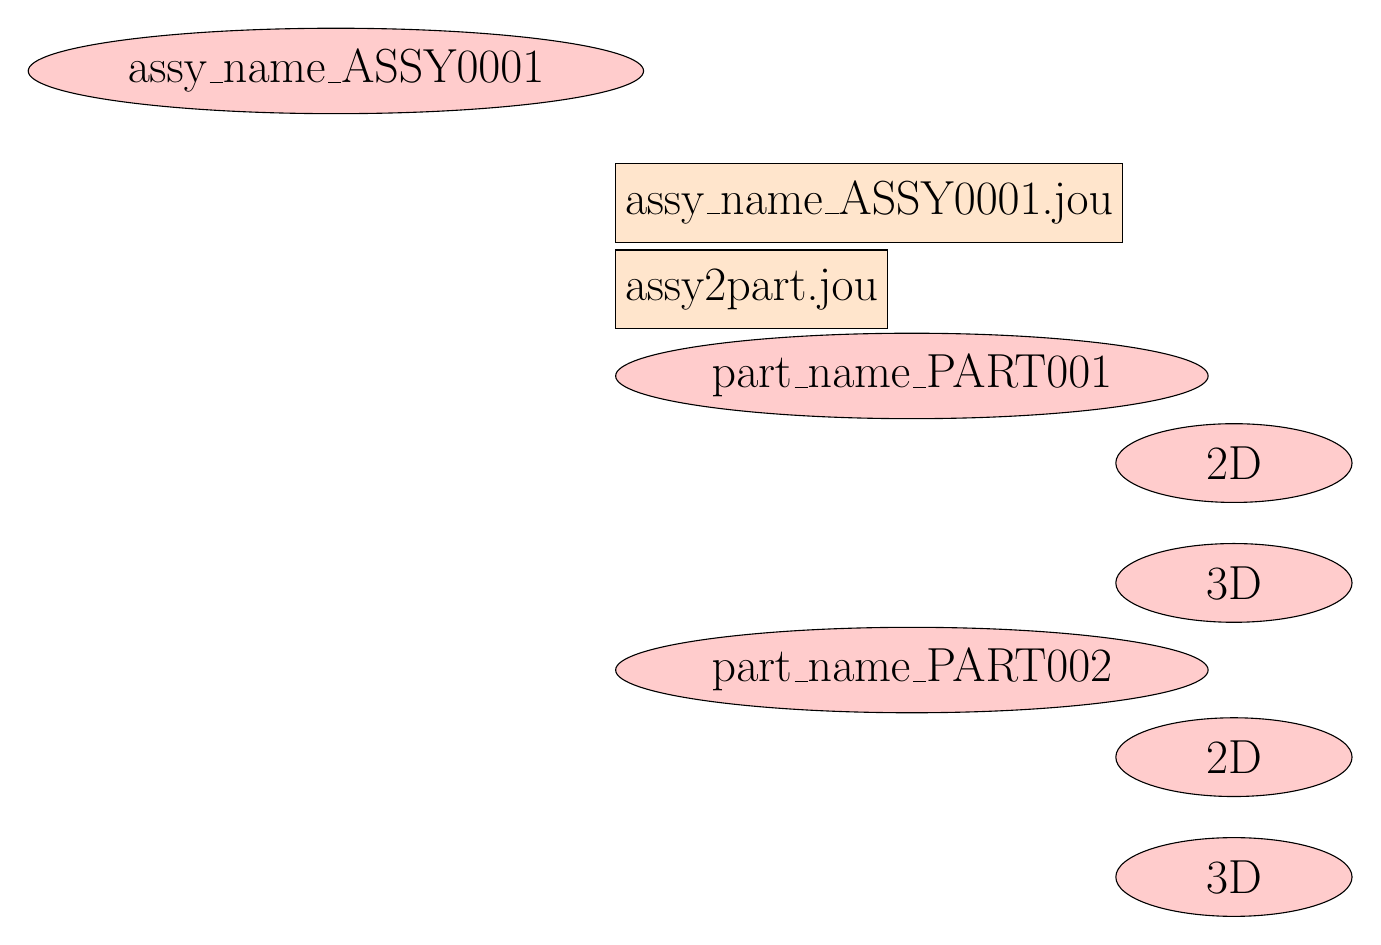
\begin{tikzpicture}[node distance=1.1cm]

%%% Nodes
\node[startstop] (maindir) {\LARGE assy\_name\_ASSY0001};
\node[process] (assyjou) [below right=of maindir] {\LARGE assy\_name\_ASSY0001.jou};
\node[process] (assy2part) [below=of assyjou.west, anchor=west] {\LARGE assy2part.jou};
\node[startstop] (partdir1) [below=of assy2part.west, anchor=west] {\LARGE part\_name\_PART001};
\begin{scope}[node distance=0.2in]
  \node[startstop] (dir2D1) [below right=of partdir1] {\LARGE 2D};
  \node[startstop] (dir3D1) [below=of dir2D1] {\LARGE 3D};
  \node[startstop] (partdir2) [below left=of dir3D1] {\LARGE part\_name\_PART002};
  \node[startstop] (dir2D2) [below right=of partdir2] {\LARGE 2D};
  \node[startstop] (dir3D2) [below=of dir2D2] {\LARGE 3D};
\end{scope}

\end{tikzpicture}

%%%%%%%%%%%%%%%%%%%%%%%%%%%%%%%%%%%%%%%%%%%%%%%%%%%%%%%%%%%%%%%%%%%%%%%%%%%%%%%
\end{document}
